\subsubsubsection{Norme progettuali}\label{normeProgettuali}
\subsubsubsubsection{Denominazione di entità e relazioni}\label{sdeer}
Tutti i package, le classi, i metodi e gli attributi devono essere denominati in modo chiaro. Il nome deve avere una lunghezza che non ne pregiudichi chiarezza e leggibilità. Le abbreviazioni ai nomi degli elementi sono ammesse soltanto se risultano immediatamente comprensibili, contestualizzate e non devono causare ambiguità. Inoltre è preferibile utilizzare sostantivi per i nomi delle entità e verbi per le relazioni.
\subsubsubsubsection{Notazioni per la progettazione architetturale}
Poiché nel linguaggio \gloxy{JavaScript} le funzioni sono costrutti \gloxy{high-order} in aggiunta al formalismo \gloxy{UML} 2.0 è stata definita una notazione apposita per rappresentare il tipo di dato funzione: \texttt{function(<parameters>)}. Questa notazione rappresenta quindi il tipo funzione che richiede i parametri \texttt{<parameters>}.\\
%Inizio parte nuova
Durante la descrizione delle componenti viene spesso utilizzata la notazione ``\textit{oggetto contenente le informazioni riguardo ... organizzate come coppie chiave/valore}'' per indicare un oggetto \gloxy{JavaScript} che ha come campi dati le varie chiavi e ognuno di questi campi ha come valore il dato associato alla chiave. \\
Ad esempio ``\textit{un oggetto contenente le informazioni riguardanti i \gloxy{percorsi} presenti all'interno di un \gloxy{progetto}, organizzate come coppie chiave/valore, usando come chiave l'id del \gloxy{percorso} e come valore il nome}'' individua un oggetto che ha come campi dati tutti gli \texttt{id} dei vari \gloxy{percorsi di presentazione} e come valore del campo è assegnato il nome del \gloxy{percorso} di presentazione.
%fine parte nuova
Per facilitare la comprensione dei diagrammi \gloxy{UML} si è scelto di utilizzare il colore arancione per evidenziare le \gloxy{librerie} esterne inoltre, quando vengono presentati i diagrammi dei package, vengono mostrate le classi prive dei campi dati e dei metodi.\\
Questa scelta è stata fatta per evitare di creare diagrammi troppo grandi che sarebbero risultati illeggibili.
I diagrammi completi di ogni classe saranno quindi presenti solo vicino alle relative descrizioni.
\subsubsubsubsection{Notazioni per la progettazione di dettaglio}
\subsubsubsubsubsection{Notazioni per il \gloxy{Front-End}}\label{std_angular}
\subsubsubsubsubsubsection{\gloxy{Controller} e \$scope}\label{notazioneControllersAngularJS}
Nella definizione dei vari controllers dell'applicazione gli oggetti che saranno definiti all'interno dello \texttt{\$scope} sono stati modellati come campi dati o metodi pubblici della classe. \\
Pertanto gli attributi e metodi definiti in un oggetto \texttt{\$scope} coincideranno con gli attributi e metodi pubblici del \gloxy{controller} al quale è associato.
Ad esempio il seguente diagramma \gloxy{UML} definisce un \gloxy{controller} che:
\begin{itemize}
\item Inserisce nello \texttt{\$scope} l'oggetto \texttt{publicString} e la funzione \texttt{publicFunction};
\item Ha un campo dati \texttt{privateString} e una funzione \texttt{privateFunction} privati, cioè visibili solamente all'interno della funzione che definisce il \gloxy{controller}.
\end{itemize}
\begin{figure}[H]
\centering
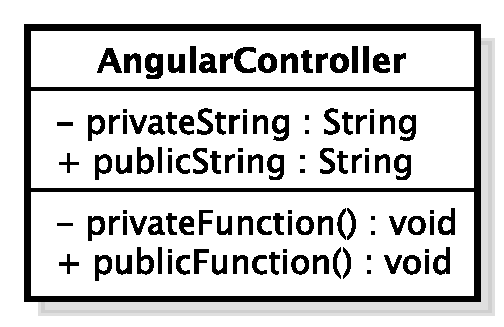
\includegraphics[width=3cm]{../immagini/angularController.pdf}
\caption{Esempio della definizione UML di un controller di Angular}
\label{fig:contorllerAngular}
\end{figure}
\FloatBarrier
\subsubsubsubsubsubsection{Directive}
Nelle descrizioni degli \textit{scope isolati} delle directive, la modalità con cui vengono passati i parametri utilizza la seguente notazione:
\begin{itemize}
\item \texttt{@:} indica che il parametro passato allo scope è una stringa e i cambiamenti effettuati su di essa dallo scope non sono visibili all'esterno;
\item \texttt{=:} indica che il parametro passato allo scope è un riferimento ad un oggetto;
\item \texttt{\&:} indica che il parametro passato è una funzione, che può avere dei parametri, e che lo scope può essere invocato dalla directive.
\end{itemize}
Come nome per l'oggetto \textit{scope} nella definizione di una directive si è scelto di utilizzare \texttt{scope} al posto di \texttt{\$scope} in quanto rispecchia il nome del campo dati utilizzato nella definizione della directive.\\
Nei diagrammi delle classi relative alle directive sono stati esplicitati solamente i campi dati, definiti da \gloxy{AngularJS}, necessari all'applicazione.
\subsubsubsubsubsubsection{Promise e \$q}
Tutti i metodi dei services che eseguono richieste al \gloxy{server} forniscono come valore di ritorno una promessa. Questo è stato modellato indicando come tipo di ritorno la classe \texttt{Promise}, maggiori informazioni riguardo l'interfaccia della classe e le \gloxy{API} offerte da \texttt{\$q} possono essere trovate nella pagina: \url{https://docs.angularjs.org/api/ng/service/$q}%$.
\subsubsubsubsubsubsection{Tipi di dato}
Per differenziare i vari tipi di dato usati forniti da \gloxy{Angular} si è scelto di utilizzare la seguente notazione:
\begin{itemize}
\item \texttt{Scope}: per i vari oggetti \texttt{\$scope};
\item \texttt{Promise}: per le promesse;
\item \texttt{DOMElement}: per gli oggetti jQuery o \gloxy{jqLite} passati alla funzione \texttt{link} di una directive;
\item \texttt{MouseEvent}: per gli oggetti jQuery che rappresentano un evento del \gloxy{browser} scatenato dal mouse dell'utente;
\item \texttt{\$nomeDelService}: per il tipo dei vari service, es: \texttt{\$http} indica il tipo del servizio \texttt{\$http}.
\end{itemize}
Maggiori informazioni riguardo le interfacce pubbliche di questi oggetti sono disponibili nella documentazione ufficiale dei \gloxy{framework}:
\begin{itemize}
\item \gloxy{AngularJS}: \url{https://docs.angularjs.org/api};
\item jQuery: \url{http://api.jquery.com}.
\end{itemize}
\subsubsubsubsubsection{Notazioni per il \gloxy{Back-End}}
Per convenzione i metodi definiti in questa componente non hanno mai tipo di ritorno. Infatti il tipo di ritorno in molti casi dipende dal comportamento \gloxy{runtime} del \gloxy{back-end}, questo può ritornare un messaggio d'errore oppure un oggetto Response contenente la risposta del \gloxy{server}.
\subsubsubsubsubsubsection{Express}
Nell'architettura definita dai \rPs si è preferito mantenere la notazione \texttt{nomeRouter} che veniva utilizzato nella versione 3 di Express, al posto di \texttt{nomeRoutes} della versione 4 di Express perché è stato ritenuto più significativo.
La motivazione di questa scelta deriva dal fatto che ogni modulo contiene tutte \textit{routes} logicamente correlate tra loro, è quindi più facile pensare ad un modulo come \textit{router} specifico anziché come un  aggregato di \textit{routes}.
Di conseguenza la cartella contenente i vari moduli di \textit{routes} si chiamerà \texttt{Routers} anziché \texttt{Routes}.
\subsubsubsubsubsubsection{\gloxy{MongoDB} e \gloxy{Mongoose}}
Come identificativo per la ricerca di oggetti nelle \texttt{collections} di \gloxy{MongoDB} vengono usati parametri di tipo \texttt{\gloxy{ObjectId}}. A livello di implementazione ai metodi con parametri di tipo \texttt{\gloxy{ObjectId}} verranno passate delle stringhe. La conversione viene effettuata automaticamente da \gloxy{Mongoose}.
